\let\negmedspace\undefined
\let\negthickspace\undefined
\documentclass[journal,12pt,onecolumn]{IEEEtran}
\usepackage{cite}
\usepackage{amsmath,amssymb,amsfonts,amsthm}
\usepackage{algorithmic}
\usepackage{graphicx}
\graphicspath{{./figs/}}
\usepackage{textcomp}
\usepackage{xcolor}
\usepackage{txfonts}
\usepackage{listings}
\usepackage{enumitem}
\usepackage{mathtools}
\usepackage{gensymb}
\usepackage{comment}
\usepackage{caption}
\usepackage[breaklinks=true]{hyperref}
\usepackage{tkz-euclide} 
\usepackage{listings}
\usepackage{gvv}                                        
%\def\inputGnumericTable{}                                 
\usepackage[latin1]{inputenc}     
\usepackage{xparse}
\usepackage{color}                                            
\usepackage{array}
\usepackage{longtable}                                       
\usepackage{calc}                                             
\usepackage{multirow}
\usepackage{multicol}
\usepackage{hhline}                                           
\usepackage{ifthen}                                           
\usepackage{lscape}
\usepackage{tabularx}
\usepackage{array}
\usepackage{float}
\newtheorem{theorem}{Theorem}[section]
\newtheorem{problem}{Problem}
\newtheorem{proposition}{Proposition}[section]
\newtheorem{lemma}{Lemma}[section]
\newtheorem{corollary}[theorem]{Corollary}
\newtheorem{example}{Example}[section]
\newtheorem{definition}[problem]{Definition}
\newcommand{\BEQA}{\begin{eqnarray}}
\newcommand{\EEQA}{\end{eqnarray}}
\newcommand{\define}{\stackrel{\triangle}{=}}
\theoremstyle{remark}
\newtheorem{rem}{Remark}

\begin{document}

\title{4.13.60}
\author{ee25btech11056 - Suraj.N}
\maketitle
\renewcommand{\thefigure}{\theenumi}
\renewcommand{\thetable}{\theenumi}

\begin{document}

\textbf{Question :} A line through $A(5,4)$ meets the lines 
$x+3y+2=0$, $2x+y+4=0$ and $x-y-5=0$ 
at $B,C,D$ respectively. If 
\[
\left(\frac{15}{AB}\right)^2 + \left(\frac{10}{AC}\right)^2 = \left(\frac{6}{AD}\right)^2,
\]
find the equation of the line.

\textbf{Solution :}

\begin{table}[h!]
  \centering
  \begin{tabular}{|c|c|}
\hline
\textbf{Name} & \textbf{Value} \\ \hline
$\vec{A}$ & $\myvec{2 & 1 \\0 & 3}$ \\ \hline
\end{tabular}

  \caption*{Table : Lines}
  \label{4.13.60}
\end{table}

Let the required line be
\begin{align}
\vec{x_4} &= \myvec{5\\4} + k\myvec{1\\m}
\end{align}

Hence the points $B,C,D$ can be written as
\begin{align}
\vec{B} &= \myvec{5\\4} + k_1\myvec{1\\m} = \myvec{5+k_1\\4+k_1m}  \\
\vec{C} &= \myvec{5\\4} + k_2\myvec{1\\m} = \myvec{5+k_2\\4+k_2m} \\
\vec{D} &= \myvec{5\\4} + k_3\myvec{1\\m} = \myvec{5+k_3\\4+k_3m} 
\end{align}

Find $k_1,k_2,k_3$\\
Since $\vec{B}$ lies on $\vec{x_1}$
\begin{align}
\myvec{\tfrac{1}{3} & 1}\vec{B} &= -\tfrac{2}{3}\\
\myvec{\tfrac{1}{3} & 1}\myvec{5+k_1\\4+k_1m} &= -\tfrac{2}{3}\\
\frac{17}{3}+\brak{m+\tfrac{1}{3}}k_1 &= -\tfrac{2}{3} \\
\brak{m+\tfrac{1}{3}}k_1 &= -\tfrac{19}{3} \\
k_1 &= \frac{-19}{3m+1}
\end{align}

\pagebreak

Since $\vec{C}$ lies on $\vec{x_2}$
\begin{align}
\myvec{2 & 1}\vec{C} &= -4 \\
\myvec{2 & 1}\myvec{5+k_2\\4+k_2m} &= -4\\
(2+m)k_2+14 &= -4 \\
(2+m)k_2 &= -18 \\
k_2 &= \frac{-18}{m+2}
\end{align}

Since $\vec{D}$ lies on $\vec{x_3}$
\begin{align}
\myvec{-1 & 1}\vec{D} &= -5\\
\myvec{-1 & 1}\myvec{5+k_3\\4+k_3m} &= -5\\
(m-1)k_3-1 &= -5 \\
(m-1)k_3 &= -4 \\
k_3 &= \frac{-4}{m-1}
\end{align}

Find distances
\begin{align}
  \norm{\vec{B}-\vec{A}} &= \norm{\myvec{k_1\\k_1m}} = |k_1|\sqrt{1+m^2} \\
\norm{\vec{C}-\vec{A}} &= \norm{\myvec{k_2\\k_2m}} = |k_2|\sqrt{1+m^2} \\
\norm{\vec{D}-\vec{A}} &= \norm{\myvec{k_3\\k_3m}} = |k_3|\sqrt{1+m^2}
\end{align}

Use the given equation
\begin{align}
\left(\frac{15}{\norm{\vec{B}-\vec{A}}}\right)^2 
+ \left(\frac{10}{\norm{\vec{C}-\vec{A}}}\right)^2 
&= \left(\frac{6}{\norm{\vec{D}-\vec{A}}}\right)^2
\end{align}

Substitute distances:
\begin{align}
\frac{225}{k_1^2(1+m^2)} + \frac{100}{k_2^2(1+m^2)} 
&= \frac{36}{k_3^2(1+m^2)}
\end{align}

Multiply throughout by $(1+m^2)$:
\begin{align}
\frac{225}{k_1^2} + \frac{100}{k_2^2} &= \frac{36}{k_3^2}
\end{align}

Substitute values of $k_1,k_2,k_3$:
\begin{align}
\frac{225}{\brak{\tfrac{-19}{3m+1}}^2} + \frac{100}{\brak{\tfrac{-18}{m+2}}^2}
&= \frac{36}{\brak{\tfrac{-4}{m-1}}^2}
\end{align}

Simplify:
\begin{align}
\frac{225(3m+1)^2}{361} + \frac{100(m+2)^2}{324} &= \frac{9(m-1)^2}{4}\\
 \end{align}

\begin{align}
  429031m^2 + 1108138m -45869 &= 0
\end{align}

\pagebreak

This gives a quadratic in $m$. Solving by using the quadratic formula, we get
\begin{align}
m &= 0.04075, \quad m = -2.62364
\end{align}

\textbf{Answer :}\\

Final equations of the line\\
For $m=0.04075$:

\begin{align}
  \vec{x_4} &= \myvec{5\\4} + k\myvec{1\\0.04075}
\end{align}

For $m=-2.62364:

\begin{align}
  \vec{x_4} &= \myvec{5\\4} + k\myvec{1\\-2.62364}
\end{align}

\pagebreak

\begin{figure}[h!]
  \centering
  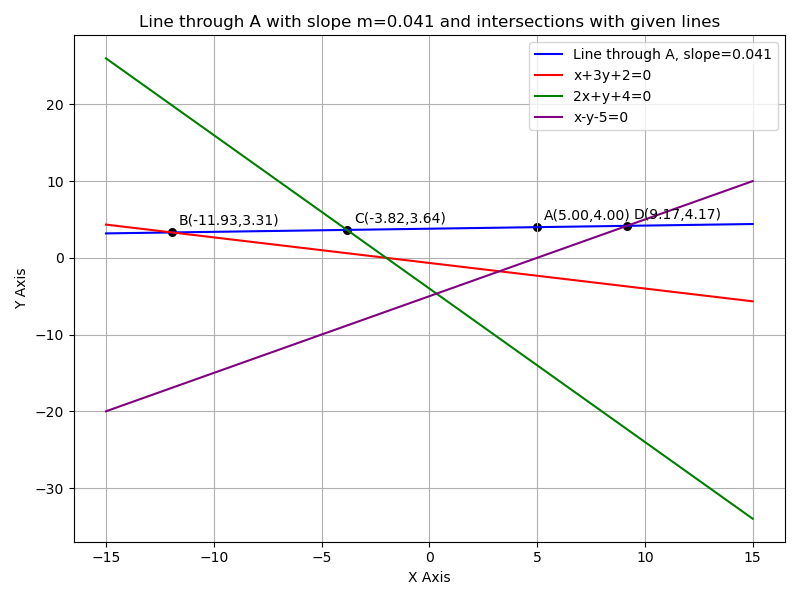
\includegraphics[width=0.7\columnwidth]{figs/lines_1.png} 
   \caption*{Fig : Lines 1}
  \label{Fig1}
\end{figure}

\begin{figure}[h!]
  \centering
  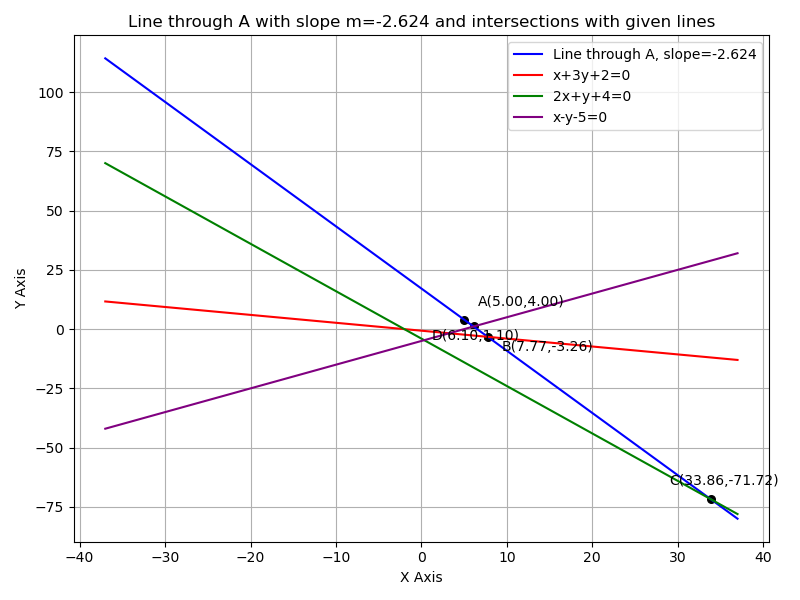
\includegraphics[width=0.7\columnwidth]{figs/lines_2.png} 
   \caption*{Fig : Lines 2}
  \label{Fig2}
\end{figure}


\end{document}

